%-----------------------------------------------------------------------------%
\chapter{\babTiga}
%-----------------------------------------------------------------------------%
Bab ini akan menjelaskan metodologi penelitian yang dilaksanakan.Bagian ini juga
menjelaskan tahapan penelitian yang dilakukan, sistem pendukung penelitian, dan data
penelitian

%-----------------------------------------------------------------------------%
\section{Tahapan Penelitian}
%-----------------------------------------------------------------------------%
\hspace{0.5cm}Tahapan dari penelitian yang dilakukan terdiri dari studi pustaka,
percobaan aplikasi, persiapan program, persiapan data, pelaksanaan penelitian dan analisis hasil
penelitian. Tahapan tersebut dapat dilihat pada gambar berikut ini
\begin{figure}
	\centering
	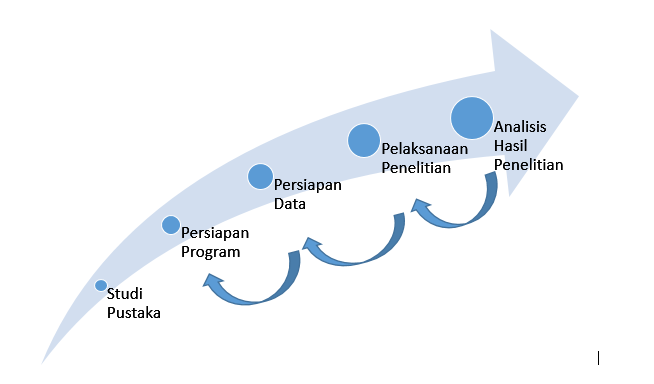
\includegraphics{workflow_skripsi.PNG}
	\caption{Tahapan Penelitian}
\end{figure}

Pada tahap studi pustaka dilakukan eksplorasi mengenai konsep penemuan obat baik secara tradisional maupun memanfaatkan IT, \textit{cloud computing} dan virtualisasi komputer berdasarkan literatur - literatur tulis yang ada. 

Dalam tahap persiapan sistem, penulis mencoba membiasakan diri dengan mengoperasikan aplikasi yang digunakan dalam penelitian, Docker dalam hal virtualisasi maupun Autodock dan Autodock Vina dalam melakukan \textit{virtual screening}. Kemudian dilakukan konfigurasi dan instalasi aplikasi tersebut. Aplikasi yang terlibat dalam penelitian ini diantaranya Autodock versi 4.2, Autodock Vina versi 1.1, dan Autodock Tools versi 1.5.2 yang akan digunakan untuk preparasi data. Selain itu Docker versi terakhir yang akan digunakan 1.5.0 sebagai platform virtualisasi komputer. Pada tahapan ini , penulis juga membuat beberapa \textit{script} sederhana yang akan digunakan untuk menjalankan aplikasi Autodock dan Autodock Vina secara otomatis dari awal pengerjaan hingga pengumpulan hasil akhir. \textit{Script} dapat dilihat pada lampiran C  untuk Autodock Vina dan lampiran D untuk Autodock. Instalasi aplikasi yang digunakan dalam penelitian ini dapat dilihat pada lampiran A.

Pada tahap pemrosesan data dilakukan \textit{pre-docking} atas data mentah
penelitian. Proses \textit{pre-docking} dilakukan sebagai syarat untuk menjalankan aplikasi Autodock 4.2 . Untuk Autodock Vina 1.1 , aplikasi dapat langsung dijalankan tanpa perlu data dipreparasi. Proses \textit{pre-docking} pada Autodock dapat dilihat pada lampiran B.

Pelaksanaan penelitian dilaksanakan pada sebuah PC desktop pada Laboratorium Jaringan Komputer lantai 5 gedung B Fasilkom UI. Kedua aplikasi tersebut dijalankan secara bergantian pada \textit{platform} Docker yang telah terpasang. Tahapan ini dapat dilakukan berulang kali hingga didapatkan data yang dapat dianalisis.

Tahap akhir dari penelitian ini adalah analisis hasil penelitian. Analisis hasil penelitian dilakukan atas data keluaran proses virtual screening. Data yang dianalisis adalah data keluaran berupa running time yang diperoleh dengan program date yang tersedia pada sistem operasi berbasis GNU/Linux.

%-----------------------------------------------------------------------------%
\subsection{Workflow Penelitian}
%-----------------------------------------------------------------------------%
\hspace{0.5cm}Alur penelitian ini diawali dengan instalasi \textit{platform} Docker pada \textit{PC desktop} yang akan digunakan. Kemudian dalam tahapan \textit{molecular docking} yang akan dilakukan dengan aplikasi Autodock dan Autodock Vina terbagi menjadi 3, yaitu \textit{pre-docking}, \textit{docking}, dan analisis hasil log \textit{docking}. Proses ini dimulai dari mengunduh \textit{ligand} dan \textit{receptor} hingga mendapatkan hasil akhir berupa log hasil \textit{molecular docking} dari aplikasi Autodock dan Autodock Vina. Berikut merupakan gambar \textit{workflow} :
\begin{figure}
		\centering
		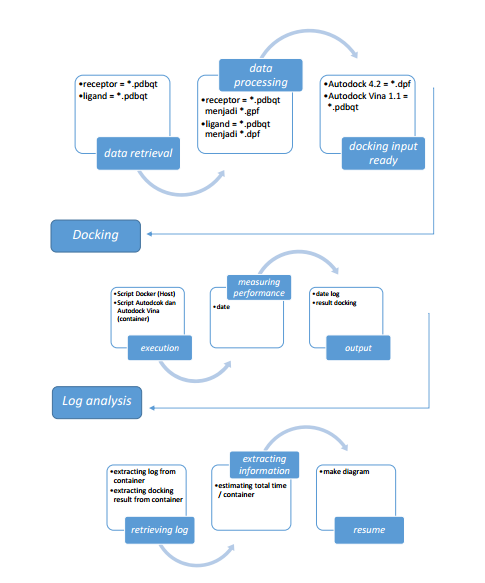
\includegraphics{workflow.PNG}
		\caption{\textit{Workflow} penelitian}
\end{figure} 

%-----------------------------------------------------------------------------%
\section{Sistem Pendukung Penelitian}
%-----------------------------------------------------------------------------%
\hspace{0.5cm}Penelitian ini menggunakan \textit{platform} Docker yang telah ter\textit{install} pada PC desktop yang terdapat pada Laboratorium Jaringan Komputer Gedung B Lantai 5 Fasilkom UI. Berikut ini merupakan spesifikasi PC desktop yang digunakan :
\begin{table}
	\centering
	\begin{tabular}{|l|l|l|l|l|}
		\hline
		\multicolumn{5}{|l|}{Spesifikasi Komputer} \\ \hline
		\multicolumn{2}{|l|}{Prosesor} & \multicolumn{3}{l|}{Intel i7-2600 CPU @ 3.40GHz X 4} \\ \hline
		\multicolumn{2}{|l|}{RAM} & \multicolumn{3}{l|}{5.8 GiB} \\ \hline
		\multicolumn{2}{|l|}{Hardisk} & \multicolumn{3}{l|}{418 GB} \\ \hline
		\multicolumn{2}{|l|}{Sistem Operasi} & \multicolumn{3}{l|}{debian 8.0} \\ \hline
		\multicolumn{2}{|l|}{Instruction Set} & \multicolumn{3}{l|}{64-bit} \\ \hline
	\end{tabular}
	\caption{Spesifikasi PC desktop}
	\label{my-label}
\end{table}
%-----------------------------------------------------------------------------%
\section{Data Penelitian}
%-----------------------------------------------------------------------------%
\hspace{0.5cm}Data yang digunakan dalam penelitian ini seluruhnya merupakan data yang diperoleh dari seorang rekan yang mengelola situs data tanaman obat Indonesia. Data yang digunakan valid dan merupakan salah satu persyaratan dalam penelitian ini untuk membandingkan hasil performa penelitian ini dengan penelitian terkait yang sebelumnya telah dilakukan. 
\subsection{Pemilihan Data}
%-----------------------------------------------------------------------------% 
\hspace{0.5cm}Data yang digunakan dalam penelitian ini diambil dari Herbaldb \cite{herbaldb}. Herbaldb merupakan situs yang menyediakan data tanaman obat Indonesia yang dimiliki oleh Fakultas Farmasi Universitas Indonesia. Data yang diperoleh telah diolah oleh Herbaldb dan jumlah data yang digunakan sebanyak 1406 data \textit{receptor} dan 1 buah data \textit{ligand}
\subsection{Pemrosesan Data}
%-----------------------------------------------------------------------------% 
\hspace{0.5cm}Data yang telah diperoleh harus menjalani proses \textit{pre-docking} sebelum dapat dilakukan \textit{virtual screening}.Pada kesempatan ini penulis telah memperoleh data \textit{ligand} dan \textit{receptor} dalam ekstensi yang sama, sehingga langkah \textit{pre-processing} hanya dilakukan pada file yang akan digunakan untuk menjalankan aplikasi Autodock versi 4.2 \cite{tutorial autodock}. Langkah \textit{pre-processing} dilakukan dengan aplikasi AutodockGrid4 yang telah ada dari instalasi Autodock versi 4.2 :
\begin{itemize}
	\item \textbf{Mempersiapkan AutoGrid Parameter Files untuk receptor} \\
	AutoGrid Parameter Files pada receptor disiapkan dengan aplikasi
	Autodock Tools 1.5.2. AutoGrid Parameter Files berisi berkas yang siap
	dipetakan atas ligand menggunakan autogrid4. Hasil dari tahapan ini adalah
	berkas receptor dalam format *.gpf
	\item \textbf{Menghitung atomic affinity maps} \\
	Pemetaan yang sudah dilakukan pada receptor dan menghasilkan
	berkas receptor dalam format *.gpf harus dipetakan untuk setiap berkas
	ligand. Proses pemetaan ini dilakukan dengan cara menghitung atomic
	affinity maps pada berkas receptor dengan menggunakan aplikasi autogrid4.
	Tahapan ini akan menghasilkan berkas pemetaan dalam format *.glg,
	*.map, *maps.xyz dan *.maps.fld.
	\item \textbf{Mempersiapkan docking parameter files untuk setiap ligand}  \\
	Tahapan terakhir adalah menyiapkan docking parameter files untuk
	setiap ligand dibantu modul phyton dari Autodock Tools 1.5.2 yang
	bernama . Docking parameter files ini berisi informasi
	terkait ligand seperti jumlah atom, koordinat atom dan jumlah torsi aktif
	yang dimiliki yang sudah dipetakan ke dalam informasi pada receptor. Hasil
	dari tahapan ini adalah berkas docking parameter files dalam format *.dpf.
\end{itemize}

Sedangkan tahapan \textit{pre-docking} pada aplikasi Autodock Vina versi 1.1 tidak perlu dilakukan lagi dikarenakan ekstensi file telah memenuhi persyaratan dalam menjalankan aplikasi tersebut. 

Berikut merupakan perbandingan tahapan \textit{pre-docking} antara Autodock versi 4.2 dan Autodocok versi 1.1
\begin{table}
	\begin{tabular}{|l|l|}
		\hline
		Autodock 4.2 & Autodock Vina 1.1 \\ \hline
		1. Mempersiapkan AutoGrid parameterfiles untuk receptor & 1.Tahap pre-docking selesai \\ \hline
		2. Menghitung atomic affinity maps & \multirow{3}{*}{\begin{tabular}[c]{@{}l@{}}Transparansi proses pre-docking\\ Autodock Vina 1.1\end{tabular}} \\ \cline{1-1}
		\begin{tabular}[c]{@{}l@{}}3. Mempersiapkan docking parameter files\\ untuk setiap ligand\end{tabular} &  \\ \cline{1-1}
		4. Tahap pre-docking selesai &  \\ \hline
	\end{tabular}
	\caption{Preparasi data pada Autodock dan Autodock Vina}
\end{table}

\section{Skenario Eksperimen Penelitian}
%-----------------------------------------------------------------------------%
Dalam penelitian ini, penulis akan melaksanakan 10 skenario eksperimen dengan 5 skenario melibatkan Autodock dan 5 skenario melibatkan Autodock Vina. Tiap - tiap skenario pada Autodock maupun Autodock vina adalah sama, yaitu menjalankan aplikasi tersebut pada \textit{platform} Docker dengan data yang telah dipreparasi. Perbedaan mendasar untuk setiap skenario adalah jumlah \textit{container} yang digunakan dan persebaran data yang ditampung oleh tiap - tiap \textit{container}. Persebaran data dapat diestimasi dengan total data \textit{receptor} yang digunakan dibagi dengan jumlah \textit{container} untuk setiap skenario. Maka untuk setiap \textit{container} akan memperoleh jumlah data yang sama (hasil bagi) dan jika tidak dapat dibagi sama rata, ada beberapa \textit{container} yang berisikan data sebanyak sisa jumlah data tersebut (modulo dari jumlah data dengan jumlah \textit{container}).
\begin{table}
	\begin{tabular}{|c|c|c|}
		\hline
		Eksperimen & Jumlah \textit{container} & Jumlah data receptor per container \\ \hline
		1 & 50 & 28 \\ \hline
		2 & 100 & 14 \\ \hline
		3 & 150 & 9 \\ \hline
		4 & 200 & 7 \\ \hline
		5 & 250 & 5 \\ \hline
	\end{tabular}
	\caption{Pembagian \textit{container} dan data setiap \textit{container}}
	\label{my-label}
\end{table}
Angka tersebut didapatkan dari percobaan yang penulis lakukan untuk mengetahui maksimum jumlah \textit{container} yang dapat dijalankan pada \textit{desktop} PC. Didapatkan angka 289 \textit{container} yang dapat dijalankan dalam 1 waktu, namun menyebabkan \textit{desktop} PC \textit{hang}. Maka penulis mencoba untuk menetapkan \textit{range container} dengan kelipatan 50 dalam skenario penelitian. 


\section{Pengukuran Kinerja}
%-----------------------------------------------------------------------------% 
Dalam mengukur kinerja penelitian ini, penulis menggunakan 1 parameter yaitu \textit{running time}. \textit{Running time} digunakan program \textit{date} yang tersedia dalam sistem operasi debian. Penulis akan mengumpulkan setiap \textit{running time} untuk masing masing \textit{container} yang dijalankan pada setiap eksperimen dan akan diolah (proses terlama, tercepat dan rata rata waktu proses). Pada bagian akhir, penulis mencoba untuk menghitung waktu proses 1 molekul untuk masing - masing skenario.




